\section{Metrology in the vicinity of Dicke states}
\label{sec:vd}
\thiswatermark{\put(1,-282){\color{l-grey}\rule{84pt}{88pt}}
\put(84,-282){\color{grey}\rule{410pt}{88pt}}}


\quotes{Robert H. Dicke}{An experimentalist should not be unduely inhibited by theoretical untidyness}

\lettrine[lines=2, findent=3pt,nindent=0pt]{I}{n} this chapter we will present recent results regarding the metrological usefulness of a family of unpolarized states.
Such states can be used as trial states to estimate the homogeneous magnetic field strength, see Section~\ref{sec:bg-quantum-magnetometry} for references about magnetometry.
It turns out that unpolarized states are the most adequate states to reach the Heisenberg limit, as it was shown in the Section~\ref{sec:bg-quantum-metrology}.
Hence, these states have attracted considerable interest.

One of the figures of merit of these states is the so-called unpolarized Dicke state \cite{Dicke1954} in an arbitrary $l$-direction, which consists of an equal number of qubits pointing in the $l$-direction and pointing opposite direction while the whole state is symmetrized, and where $l=x,y,z$.
It can be written as
\be
   \ket{\dicke{N}}_l\equiv \ket{\dicke{N,\frac{N}{2}}}_l:= \binom{N}{N/2}^{-\frac{1}{2}}
  \sum_{k\in \sigma_\text{s}}
  \mathcal{P}_{k} \left( \ket{1}_l^{\otimes N/2} \ket{0}_l^{\otimes N/2}
  \right),
  \label{eq:vd-unpolarized-dicke}
\ee
where $k$ are elements of the set of all possible unique permutations of $N$ elements of 2 kinds, $\sigma_\text{s}$, see Appendix~\ref{app:angular-subspaces} for more information about the notation used in Eq.~\eqref{eq:vd-unpolarized-dicke}.
Note that in Eq.~\eqref{eq:vd-unpolarized-dicke} we omit the subscript giving the number of $\ket{1}$'s which is the notation we will follow in this chapter.
Such a state is known to be highly entangled \cite{Toth2007, Toth2009a} and can reach Heisenberg scaling when used for magnetometry \cite{Holland1993}.

One of the characteristics of state Eq.~\eqref{eq:vd-unpolarized-dicke} is that it is an eigenstate of the collective operator $J_l$ with corresponding eigenvalue equal to zero.
At the same time, it lives in the subspace where the collective total spin is maximum, i.e, $\expect{\bs{J}^2}=N(N+2)/4$.
Based on these and the fact that the state is unpolarized, we can see that has a very large uncertainty for the collective spin operators perpendicular to $J_l$.

For metrology, we chose the magnetic field to be pointing in the $z$-axis.
Hence, the Dicke state we choose must an eigenstate of a perpendicular component of the angular momentum operator such as $J_x$.
Hence, we will consider a scheme in which the state is rotated around the $z$-direction and the rotation angle must be estimated based on collective measurements.
A criterion to detect the metrological usefulness of states of this type has been derived in Ref.~\cite{Zhang2014}.

In this chapter, we present a condition for metrological usefulness for the case when the second moment of a total angular momentum component is measured to obtain an estimate for the rotation angle.
Our method is expected to simplify the experimental determination of metrological sensitivity since it is much easier to measure the collective operators of the state than carrying out the metrological procedure and measure directly the sensitivity.
We also test our approach using the experimental results of Refs.~\cite{Luecke2011, Krischek2011}, which realize parameter estimation with a Dicke state.
Thus, our work is expected to be useful for similar experiments in the future.

The chapter is organized as follows.
In Section~\ref{sec:vd-unpolarized-states-magnetometry}, we review some important concepts behind the theory of metrology with unpolarized states.
In Section~\ref{sec:vd-evolution-of-the-expectation-values}, we present our criterion.
In Section~\ref{sec:vd-comparison-with-qfi}, we compare findings to sensitivity bounds obtained from the quantum Fisher information.
In Section~\ref{sec:vd-testing-with-experimental-data}, we show how to apply our criterion to experimental results.

\subsection{Unpolarized Dicke states for magnetometry}
\label{sec:vd-unpolarized-states-magnetometry}

The use of unpolarized states for magnetometry has been shown useful in Eq.~\eqref{eq:bg-unpolarize-states-are-better}.
While the quantum Fisher information would give us directly the performance of the state, we typically cannot compute it because a complete knowledge of the state would be necessary, see Eq.~\eqref{eq:bg-qfi-definition-eigen-decomposition}.
On the other hand, we can use the error propagation formula Eq.~\eqref{eq:bg-error-propagation-formula} to obtain a bound on the achievable precision which at the same time bounds the QFI.

As one can see in Figure~\ref{fig:vd-secuence-evo}, a pure Dicke state of 16 qubits, initially an eigenstate of the $J_x$ operator, is rotated around the $z$-axis.
\begin{figure}[htp]
  \centering
  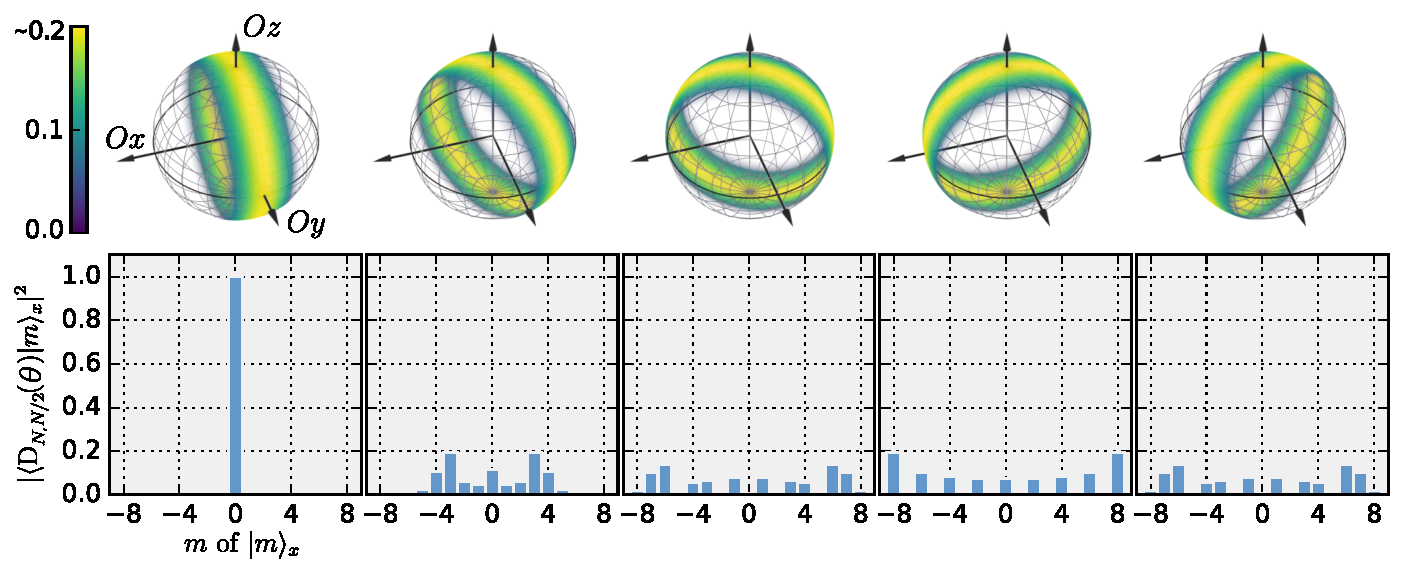
\includegraphics[scale=.65]{img/VD_evolution_of_dicke.pdf}
  \caption[Sequence of Dicke state evolution]{Sequence of the evolution of an unpolarized Dicke state of 16 qubits for $\theta=\{i\pi/6\}_{i=0}^4$. Bloch spheres representing the Husimi quasi-probabilistic distribution of the state, and below PDF of the $J_x$ positive-operator valued measure (POVM) for each step of the sequence}
  \label{fig:vd-secuence-evo}
\end{figure}
The state is unpolarized so the expectation value of any component of the total angular momentum remains zero.
It turns out that measuring the evolution of the second moment of $J_x$ allows the estimation of rotation angle $\theta$, and therefore, the magnetic field.
The expectation value $\expect{J_x^2}$ is initially zero for a pure unpolarized Dicke state, and it increases rapidly as it can be seen in the Figure~\ref{fig:vd-secuence-evo}.
Another observation is that for $\theta=\pi/2$ the value of $\expect{J_x^2}$ will be at its maximum proportional to $\expect{\bs{J}^2}$ or equivalently to $\mathcal{J}_{N/2}$, see Eq.~\eqref{eq:app-maximum-total-angular-momentum}.
Hence, the change in the second moment over the phase shift must be in this case proportional to $N^2$.
We lead to the conclusion that one only needs to measure the second moment of the collective spin $J_x$ to achieve Heisenberg scaling for the estimation.

In certain situations, it is better to use Eq.~\eqref{eq:bg-error-propagation-formula} rather than Eq.~\eqref{eq:bg-quantum-cr-bound} for calculating the achievable precision, since it gives the precision for a particular operator to be measured in an experimental setup.
This is reasonable, since in a typical experiment, only a restricted set of operators can be measured.
In this work, we will consider many-particle systems in which the particles cannot be accessed individually, and only collective quantities can be measured.
As we said, measuring the second moment of $J_x$ is a valid choice to estimate the rotation angle.
In the following equation, we show the error propagation formula when measuring the second moment of the $J_x$ total angular momentum component,
\be
  \varinv{\theta} = \frac{|\partial_{\theta} \expect{J_x}|^2}{\varian{J_x^2}}.
  \label{eq:vd-error-propagation}
\ee

Since Eq.~\eqref{eq:vd-error-propagation} is always smaller than $\qfi$, and as a consequence of Eq.~\eqref{eq:bg-entanglement-criterion-qfi}, if
\be
  \frac{|\partial_{\theta} \expect{J_x}|^2}{\varian{J_x^2}}\geqslant N
\ee
holds, then the system is entangled.
Hence again, entanglement is required for a large metrological precision.
Based on Eq.~\eqref{eq:bg-entanglement-depth-for-qfi}, we can bound the entanglement depth from below of the systems as follows.
Similarly to the previous paragraph, if for a quantum state
\be
  \frac{|\partial_{\theta} \expect{J_x}|^2}{\varian{J_x^2}}\geqslant kN
\ee
holds, then it is at least $(k+1)$-entangled.

\subsection{Evolution of the expectation values}
\label{sec:vd-evolution-of-the-expectation-values}
With the aim of obtaining the precision, Eq.~\eqref{eq:vd-error-propagation}, we will compute the dependence on $\theta$ of the expectation value of the operator $J_x$ and higher order moments.
We will use the Heisenberg picture, where the operators evolve in time while the state remains the same.
The operator $J_x$ can be written as a function of $\theta$ in the following way,
\be
  J_x(\theta) = e^{i \theta J_z} J_x(0) e^{-i \theta J_z} = J_x(0) \text{c}_\theta - J_y(0) \text{s}_{\theta},
\ee
where $J_l(0)$ for $l=x,y,z$ are the collective angular momentum operators at time equal zero.
We will denote them by $J_l$ from now on.
The notation for the trigonometric functions $\text{c}_\theta$ and $\text{s}_\theta$ was introduced in Section~\ref{sec:bg-metrology-with-almost-polarized}.

We need to compute the second and the fourth moments of $J_x$ as it is required by the Eq.~\eqref{eq:vd-error-propagation}.
But before any calculation we will make a simplifying assumption which turns out to be true in the most common situations.
The assumption is that both expectation values are even functions of $\theta$, so
\be
  \begin{split}
    \expect{J_x^2(\theta)} &=\expect{J_x^2(-\theta)}, \\
    \expect{J_x^4(\theta)} &=\expect{J_x^4(-\theta)}
  \end{split}
  \label{eq:vd-even-f-constraint}
\ee
holds.
This way we can omit the terms that are odd in $\theta$.
In Section~\ref{sec:vd-testing-with-experimental-data}, we will see that unitary dynamics of some experimentally prepared states have this property.
The assumption Eq.~\eqref{eq:vd-even-f-constraint} is needed to obtain a closed formula for the precision of the phase estimation.

The square of $J_x$ in the Heisenberg picture is written as
\be
  J_x^2(\theta)= J_x^2 \text{c}_\theta^2 + J_y^2 \text{s}_\theta^2
  - (J_xJ_y + J_yJ_x) \text{c}_\theta\text{s}_\theta.
  \label{eq:vd-evolution-of-jx2}
\ee
Hence, due to the first constraint of Eq.~\eqref{eq:vd-even-f-constraint} and Eq.~\eqref{eq:vd-evolution-of-jx2}, we require that
\be
  \expect{\{J_x,J_y\}} = 0,
  \label{eq:vd-init-2nd-constraint}
\ee
where $\{\, ,\,\}$ stands for the anticommutator.
Apart for been simpler to compute the Eq.~\eqref{eq:vd-init-2nd-constraint} is based also on initial expectation values of the state.
We will see that as we said before this is easily guarantied for most important cases.

As we have done with the expectation value of the square of $J_x$, now we  do the same for $J_x^4$.
This way one will be able to distinguish which other expectation value of combination of operators must vanish in order to have Eq.~\eqref{eq:vd-even-f-constraint} guarantied.
The fourth power of $J_x$ can be written in the Heisenberg picture as
\begin{multline}
  J_x^4(\theta)= J_x^4 \text{c}_\theta^4 + J_y^4 \text{s}_\theta^4
  + (J_x^2J_y^2 + J_xJ_yJ_xJ_y + J_xJ_y^2J_x + J_yJ_xJ_yJ_x + J_yJ_x^2J_y + J_y^2J_x^2) \text{c}_\theta^2\text{s}_\theta^2 \\
  -(J_x^3J_y+J_x^2J_yJ_x+J_xJ_yJ_x^2+J_yJ_x^3)\text{c}_\theta^3\text{s}_\theta
  -(J_xJ_y^3+J_yJ_xJ_y^2+J_y^2J_xJ_y+J_y^3J_x)\text{c}_\theta\text{s}_\theta^3.
\end{multline}
And again assuming that the expectation value of $J_x^4(\theta)$ must be an even function of $\theta$, we see that the terms multiplied by $\coss{\theta}^3\sins{\theta}$ and $\coss{\theta}\sins{\theta}^3$, respectively, must be zero.
So, the expectation value of $(J_x^3J_y+J_x^2J_yJ_x+J_xJ_yJ_x^2+J_yJ_x^3)$ and $(J_xJ_y^3+J_yJ_xJ_y^2+J_y^2J_xJ_y+J_y^3J_x)$ must vanish.
Hence, the second constraint of the Eq.~\eqref{eq:vd-even-f-constraint} can be fulfilled if
\be
  \begin{split}
    \expect{\big\{J_x^2 , \{ J_x,J_y\}\big\}}=0,\\
    \expect{\big\{J_y^2 , \{ J_x,J_y\}\big\}}=0.
  \end{split}
\ee

Finally, we can write the evolution of second and fourth moments of the $J_x$ operator as
\begin{align}
  \expect{J_x^2(\theta)}=\; &\expect{J_x^2} \text{c}_\theta^2 + \expect{J_y^2} \text{s}_\theta^2
  \label{eq:vd-evo-2nd-moment}\\
  \begin{split}
    \expect{J_x^4(\theta)}=\; &
    \expect{J_x^4}\text{c}_\theta^4 + \expect{J_y^4} \text{s}_\theta^4 \\
    & + \expect{\{J_x^2,J_y^2\}+\{J_x,J_y\}^2} \text{c}_\theta^2\text{s}_\theta^2.
  \end{split}
\end{align}
From here, we are able to write the evolution of the variance of the second moment when Eq.~\eqref{eq:vd-even-f-constraint} is fulfilled.
We obtain
\be
  \begin{split}
    \varian{J_x^2(\theta)} &= \expect{J_x^4(\theta)} -\expect{J_x^2(\theta)}^2 \\
    &= \expect{J_x^4}\text{c}_\theta^4 + \expect{J_y^4} \text{s}_\theta^4
    + \expect{\{J_x^2,J_y^2\}+\{J_x,J_y\}^2} \text{c}_\theta^2\text{s}_\theta^2
    - \big(\expect{J_x^2} \text{c}_\theta^2 + \expect{J_y^2} \text{s}_\theta^2\big)^2\\
    &= \big(\expect{J_x^4}-\expect{J_x^2}^2\big)\text{c}_\theta^4
    + \big(\expect{J_y^4}-  \expect{J_y^2}^2\big)\text{s}_\theta^4
    + \big(\expect{\{J_x^2,J_y^2\}+\{J_x,J_y\}^2} - 2 \expect{J_x^2}\expect{J_y^2}\big)
    \text{c}_\theta^2\text{s}_\theta^2\\
    &=\varian{J_x^2}\text{c}_\theta^4 + \varian{J_y^2} \text{s}_\theta^4+ \big(\expect{\{J_x^2,J_y^2\}+\{J_x,J_y\}^2} - 2 \expect{J_x^2}\expect{J_y^2}\big)\text{c}_\theta^2\text{s}_\theta^2.
  \end{split}
\ee

In order to compute the Eq.~\eqref{eq:vd-error-propagation}, we also need the modulus square of the derivative of the second moment of the $J_x$ operator.
Using Eq.~\eqref{eq:vd-evo-2nd-moment} for the expression of the evolution of the second moment, the numerator of Eq.~\eqref{eq:vd-error-propagation} follows
\be
  \begin{split}
    |\partial_\theta \expect{J_x^2(\theta)}|^2 & = |-2\expect{J_x^2}\text{c}_\theta\text{s}_\theta+2\expect{J_y^2}\text{c}_\theta\text{s}_\theta|^2\\
    & = 4\expect{J_y^2-J_x^2}^2\text{c}_\theta^2\text{s}_\theta^2.
  \end{split}
\ee

From the equations above directly follows expression for the precision of $\theta$,
\be
\begin{split}
  \varian{\theta} & = \frac{\varian{J_x^2}\text{c}_\theta^4 + \varian{J_y^2} \text{s}_\theta^4+ \big(\expect{\{J_x^2,J_y^2\}+\{J_x,J_y\}^2} - 2 \expect{J_x^2}\expect{J_y^2}\big)\text{c}_\theta^2\text{s}_\theta^2}
  {4\expect{J_y^2-J_x^2}^2\text{c}_\theta^2\text{s}_\theta^2}\\
  & = \frac{\varian{J_x^2}\text{t}_\theta^{-2} + \varian{J_y^2} \text{t}_\theta^2+ \expect{\{J_x^2,J_y^2\}+\{J_x,J_y\}^2} - 2 \expect{J_x^2}\expect{J_y^2}}
  {4\expect{J_y^2-J_x^2}^2}.
\end{split}
\label{eq:vd-result-before-simp}
\ee
To this calculations further computations follows mainly regarding to the following expectation value $\expect{\{J_x^2,J_y^2\}+\{J_x,J_y\}^2}$.
This calculus is left for the Appendix~
ef{app:simplification-of-4th-moments}.
Finally, the expression Eq.~\eqref{eq:vd-result-before-simp} can be written as
\be
  \varian{\theta} = \frac{\varian{J_x^2}\text{t}_\theta^{-2} + \varian{J_y^2} \text{t}_\theta^2 + 4\expect{J_y^2} - 3 \expect{J_z^2} - 2\expect{J_x^2}(1+\expect{J_y^2}) + 6\expect{J_xJ_y^2J_x}}
  {4\expect{J_y^2-J_x^2}^2}.
  \label{eq:vd-precision-as-theta}
\ee

We have verified the correctness of our analytic formula Eq.~\eqref{eq:vd-precision-as-theta} comparing it with a numerical simulation of the Eq.~\eqref{eq:vd-error-propagation} for the ground-state of $H=J_x^2+J_y$ for 6 qubits, $|\text{GS}\rangle$.
We computed the evolution of the expectation values of the second and the fourth moments of the operator $J_x$ for $\theta \in [0,\pi]$, for thousand of equidistant points, from which we obtained the bound, see Figure~\ref{fig:vd-evolution-of-precision}~(a).
Finally, we have also checked that the constraints assumed at the beginning of this section are fulfilled.
For that, we considered the range $\theta \in [-\pi,\pi]$ and we have computed the expectation values, see Figure~\ref{fig:vd-evolution-of-precision}~(b).
We can conclude saying that our formula Eq.~\eqref{eq:vd-precision-as-theta} reproduces exactly the evolution of the error propagation formula, Eq.~\eqref{eq:vd-error-propagation}.
\begin{figure}[htp]
  \centering
  \igwithlabel{(a)}{scale=.65}{img/VD_simulation.pdf}
  \igwithlabel{(b)}{scale=.65}{img/VD_parity_simulation.pdf}
  \caption[(a) Evolution of $\varinv{\theta}/N$. (b) Evolution of the expectation values]{(a) Evolution of the precision $\varinv{\theta}/N$ for 6 qubits based on the simulation of the system $\ket{\text{GS}}$ and its expectation values.
  The agreement with the Eq.~\eqref{eq:vd-precision-as-theta} is shown in the inset plot where the square of the difference between two approaches are plotted, the analytically obtained result and the simulation.
  The difference is more or less two orders of magnitude below the actual value for the relevant points, which is mainly because of computing the derivative near the points on which the value of the expectation value $\expect{J_x^2}$ and the value of the $\varian{J_x^2}$ are both close to zero.
  (b) With the system at hand, we verified the parity with respect to $\theta$ of the expectation values of the second and the fourth moment, so to fulfill the constraint Eq.~\eqref{eq:vd-even-f-constraint}.}
  \label{fig:vd-evolution-of-precision}
\end{figure}

\subsubsection{The optimal precision}
First of all, note that all the dependence on the phase shift $\theta$ is in the first two terms of the numerator of Eq.~\eqref{eq:vd-precision-as-theta}.
Hence, one can minimize the sum on the first two terms in order to find where the precision is best.
So it follows that for the optimal angle
\be
  \label{eq:vd-optimal-phase}
  \tan^2(\theta_{\text{opt}}) = \sqrt{\frac{\varian{J_x^2}}{\varian{J_y^2}}}
\ee
holds.
By substituting Eq.~\eqref{eq:vd-optimal-phase} into Eq.~\eqref{eq:vd-precision-as-theta}, we obtain the optimal bound as
\be
  \varian{\theta}_{\text{opt}} = \frac{\sqrt{\varian{J_x^2} \varian{J_y^2} } + 4 \expect{J_y^2} - 3 \expect{J_z^2} - 2\expect{J_x^2}(1+\expect{J_y^2}) + 6\expect{J_xJ_y^2J_x}}
  {4\expect{J_y^2-J_x^2}^2}.
  \label{eq:vd-precision}
\ee.

We conclude this section checking our bound for pure unpolarized Dicke state aligned with the $x$-axis, $\ket{\dicke{N}}_x$, whose precision bound is well known using the QFI for pure states Eq.~\eqref{eq:bg-qfi-for-pure-states},
\be
  \qfif{\ket{\dicke{N}}_x, J_z} = 4\varian{J_z}_{\ket{\dicke{N}}_x}=\frac{N(N+2)}{2}.
  \label{eq:vd-qfi-for-pure-dicke}
\ee
With this aim we compute all the expectation values needed for the Eq.~\eqref{eq:vd-precision} which almost all of them are trivial, $\expect{J_xJ_y^2J_x}=\expect{J_x^4}=\expect{J_x^2}=0$ since the state is an eigenstate of $J_x$ with an eigenvalue zero.
The last expectation value is obtained as
\be
  \expect{J_y^2} = \expect{J_z^2} = \frac{N (N+2)}{8}.
  \label{eq:vd-2moment-pure-dicke}
\ee
Note that for the Eq.~\eqref{eq:vd-2moment-pure-dicke} we use that the state is invariant under rotations over the $x$-axis, the sum of all the second moments must give $\expect{\bs{J}^2} = \frac{N (N+2)}{4}$, and $\expect{J_x^2}=0$.
Hence, the Eq.~\eqref{eq:vd-2moment-pure-dicke} holds.

From the equation above and using the expression for the optimal precision Eq.~\eqref{eq:vd-precision}, one arrives at the following formula for the precision of the phase shift for a pure unpolarized Dicke state,
\be
  \varian{\theta}_{\text{opt}} = \frac{2}{N(N+2)},
\ee
which coincides exactly with the inverse of the quantum Fisher information for such state Eq.~\eqref{eq:vd-qfi-for-pure-dicke} \cite{Luecke2011}.
Hence for the ideal Dicke state, the Cramér-Rao bound Eq.~\eqref{eq:bg-quantum-cr-bound} is saturated, which means that estimating the phase shift $\theta$ using the measurement of $\expect{J_x^2}$ is optimal.
Based on Eq.~\eqref{eq:vd-optimal-phase}, we add that the optimal angle for the ideal Dicke state is $\theta_{\text{opt}}=0$.

\subsection{Testing the formula against some known states}
\label{sec:vd-comparison-with-qfi}

In this section, we will compare our criteria based on few expectation values against the corresponding quantum Fisher information obtained for some known states.
We find that our formula gives a good lower bound on the quantum Fisher information, which is the best achievable precision when any measurement is allowed.
However note that the Cramér-Rao bound might be impractical.

Let us consider first the spin-squeezed states.
Those states will be defined as the ground states $\ket{\text{GS}}_\lambda$ of the following Hamiltonian, called the spin-squeezing Hamiltonian
\be
  H_\lambda = J_x^2 - \lambda J_y,
  \label{eq:vd-ss-hamiltonian}
\ee
see Appendix~\ref{app:spin-squeezing-hamiltonian}.
For $\lambda>0$, the ground state is unique, and it is in the symmetric subspace.
Hence, we can restrict our attention to this subspace for our computations, and hence we can model larger systems.
For $\lambda\rightarrow\infty$, the ground state is the totally polarized state in the $y$-direction Eq.~\eqref{eq:bg-totally-polarized}.
And for $\lambda\rightarrow 0^{+}$, it is the Dicke state Eq.~\eqref{eq:vd-unpolarized-dicke}.
Note that for $\lambda=0$ the eigenvalue is degenerate, so there are more than one ground states.
On the other hand, we still can use limit in which $\lambda$ tends to zero from the positive axis to arrive at the Dicke state.
Figure~\ref{fig:vd-comparing-the-bounds}~(a) shows the sensitivity we obtained together with the QFI for the same states.
Our bound is close to the QFI when the state is well polarized.
It also coincides with the bound in the $\lambda\rightarrow 0^{+}$ limit, when the ground state is close to the unpolarized Dicke state.
\begin{figure}[htp]
  \centering
  \igwithlabel{(a)}{scale=.65}{img/VD_against_spsq.pdf}
  \igwithlabel{(b)}{scale=.65}{img/VD_against_therm.pdf}
  \caption[Bound against known QFIs for different states.]{Comparison between our formula for the precision and the QFI for different states. (a) Comparison for ground states of $H_\lambda$. (b) Comparison with gaussian mixture of Dicke states.}
  \label{fig:vd-comparing-the-bounds}
\end{figure}

The second family of states we use to test our formula are the Gaussian mixture of Dicke states around the unpolarized Dicke state,
which have the following form as function of $T$ as
\be
  \rho_{T} \propto \sum_{m=0}^{N} e^{- \frac{(m+N/2)^2}{T}} \ket{\dicke{N,m}}_x\bra{\dicke{N,m}}_x
\ee
for even $N$, where $\ket{\dicke{N,m}}$ is defined in Eq.~\eqref{eq:app-definition-of-dicke-states}.
It can be used to model a noisy or thermal unpolarized Dicke state.
For $T=0$, we obtain the pure unpolarized Dicke state.
For $T>0$, other symmetric Dicke states in the vicinity of the unpolarized one are also populated.
The result can be seen in Figure~\ref{fig:vd-comparing-the-bounds}-(b).
Again, our bound seems to be quite close to the corresponding QFI.

Note also that in Figure~\ref{fig:vd-comparing-the-bounds}, based on Eq.~\eqref{eq:bg-entanglement-depth-for-qfi}, if the bound turns to be greater than $k$ integer, then a metrologically useful $(k+1)$-particle entanglement is detected in the system.
Note that this is true whenever $k$ is a divisor of $N$, or $k\ll N$.

Although showing how the optimal precision formula behaves compared with the quantum Fisher information for those two families of states, we will now prove that they indeed they fulfill the constraints appearing in Eq.~\eqref{eq:vd-even-f-constraint}.
Hence, we compute the Eq.~\eqref{eq:vd-even-f-constraint} for the spin-squeezed states $\ket{\text{GS}}_{\lambda}$.
For that it is enough to know that since those states are non-degenerate eigenvalue must preserve the symmetries of the Hamiltonian.
In this case, the Hamiltonian Eq.~\eqref{eq:vd-ss-hamiltonian} is invariant under $x\leftrightarrow -x$ and $z\leftrightarrow -z$, thus it must be invariant under $n\pi$ angle rotations under the $y$-axis for $n$ integer, for more references about symmetries in quantum mechanics see Refs. \cite{Sakurai2010, Cohen-Tannoudji1977}.
Hence, we can write for the evolution of the expectation value of any power of the $J_x$ that
\be
  \tr(e^{+i\theta J_z}J_x^m e^{-i\theta J_z} \rho_{\lambda}) = \tr(e^{+i\theta J_z}J_x^m e^{-i\theta J_z} e^{-in\pi J_y}\rho_{\lambda}e^{+in\pi J_y}),
\ee
where $\rho_{\lambda}=\ketbra{\text{GS}}{\text{GS}}_{\lambda}$.
If the equation above holds, then for the case $n=1$, we can use the cyclic property of the trace to arrive at
\be
\begin{split}
  \tr(e^{+i\pi J_y}e^{+i\theta J_z}J_x^m e^{-i\theta J_z} e^{-i\pi J_y}\rho_{\lambda}) & =
  \tr(e^{+i \theta (-1)J_z}(-1)^m J_x^m e^{-i\theta (-1) J_z}\rho_{\lambda})\\
  & = \tr(e^{-i \theta J_z}(-1)^m J_x^m e^{+i\theta J_z}\rho_{\lambda}),
\end{split}
\ee
or equivalently
\be
  \expect{J_x^m(\theta)}_{\rho_\lambda}=\expect{(-1)^m J_x^m(-\theta)}_{\rho_\lambda},
\ee
which implies that for even $m$, and specially for $m=2,4$, the expectation values are an even function of $\theta$, and that for odd $m$ the expectation values are odd functions of $\theta$, which proves the Eq.~\eqref{eq:vd-even-f-constraint} for the present case.

On the other hand for the thermal state $\rho_T$, we have that its eigenstates are simultaneously eigenstates of $J_x$, and hence the state invariant under rotations around the $x$-axis.
Which still holds for the entire state, since it is a statistical mixture of states invariant under rotations around the $x$-axis.
Moreover, it is also invariant for the case in which the state is rotated around the $x$-axis by $\pi$ angle.
Hence, we have for the evolved expectation values of $J_x^m$ that
\be
  \tr(e^{+i\theta J_z}J_x^m e^{-i\theta J_z}\rho_T) = \tr(e^{+i\theta J_z}J_x^m e^{-i\theta J_z} e^{-i \pi J_x} \rho_T e^{+i \pi J_x})
\ee
for any $m$.
Finally, using again the cyclic properties of the trace, we flip the signs of the of angular momentum components orthogonal to $J_x$, so in this case $J_y \rightarrow - J_x$ and $J_z \rightarrow -J_z$, and we arrive at
\be
  \tr(e^{+i \pi J_x} e^{+i\theta J_z}J_x^m e^{-i\theta J_z} e^{-i \pi J_x} \rho_T) =  \tr(e^{-i\theta J_z}J_x^m e^{+i\theta J_z} \rho_T).
\ee
We conclude that for this case all the moments of the $J_x$ operator are even functions of $\theta$ for the thermal state, i.e., $\expect{J_x^m(\theta)}_{\rho_{T}}=\expect{J_x^m(-\theta)}_{\rho_{T}}$, which proves that the Eq.~\eqref{eq:vd-even-f-constraint} holds for this case too.

\subsection{Using our method with real experimental data}
\label{sec:vd-testing-with-experimental-data}

In reference \cite{Luecke2014}, a state is produced in the laboratory with the proper characteristics of an unpolarized Dicke state, small variance in one direction, say $x$, and a very large variance in the perpendicular directions to the $x$-axis.
In the cited experiment with $N$ qubits, it is possible to determine the operator $J_x$ as the population imbalance of the two levels as
\be
  J_z = \frac{1}{2}(N_{+}-N_{-}),
\ee
where $N_m$ is the number of particles in the state $\ket{m}$, in this case either $\ket{+}$ or $\ket{-}$.
Hence, measuring the population imbalance and collecting the statistics of the measurements, the expectation values of all moments of $J_x$ can be obtained.
In practice, it is possible to measure the lower order moments like $\expect{J_x^2}$ and $\expect{J_x^4}$, while higher order moments need too many repetitions of the experiment to collect enough statistics.

The other two global operators $J_y$ and $J_z$ are obtained by rotating the system using a $\frac{\pi}{2}$ microwave coupling pulse before the measurement of the population imbalance.
Whether $J_y$ or $J_z$ is obtained depends on the relation between the microwave phase and the phase of the initial BEC.
The condensate phase represents the only possible phase reference in analogy to the local oscillator in optics.
Intrinsically, it has no relation to the microwave phase, such that it homogeneously average over all possible phase relations.
From another point of view, one can also say that the fluctuation of the magnetic field results in a random rotation of the spin around the $z$-axis.
Hence, what is obtained in this case is
\be
  J_\alpha = \sin(\alpha) J_y + \cos(\alpha) J_z,
\ee
where $\alpha$ is an angle, and we need to consider the average over all possible angles.
Effectively, the state has the following form
\be
  \rho = \frac{1}{2\pi}\int e^{-i\alpha J_x} \rho_0 e^{i\alpha J_x}\, \text{d}\alpha,
  \label{eq:vd-rotational-invariant-state}
\ee
where $\rho_0$ is what we would obtain if we would have access to the phase reference.
Note that the integration over the rotation angle $\alpha$ does not create entanglement.
If the state $\rho$ is entangled then $\rho_0$ has to be also entangled.

Let us see the consequences of our state having the form  Eq.~\eqref{eq:vd-rotational-invariant-state}.
For the density matrix $\rho$, since it is invariant under rotations around the $x$-axis, we have
\be
  \expect{J_\alpha^m}=\expect{J_y^m}=\expect{J_z^m}
\ee
for all $m$.
Hence the expectation values of $\expect{J_y^m}$ and $\expect{J_z^m}$ can be obtained from the statistics of measuring $J_\alpha$.
Moreover, for states of the form Eq.~\eqref{eq:vd-rotational-invariant-state} the unitary dynamics will fulfill the condition Eq.~\eqref{eq:vd-even-f-constraint}.

There is a single remaining term in the expression for the achievable precision Eq.~\eqref{eq:vd-precision}, the expectation value for $\expect{J_xJ_y^2J_x}$, which can be bounded as
\be
\begin{split}
  \expect{J_xJ_y^2J_x} &= \frac{\expect{J_x (J_y^2 + J_z^2)J_x}}{2}
  =\frac{\expect{J_x (J_x^2 + J_y^2 + J_z^2 )J_x} - \expect{J_x^4}}{2} \\
  & \leqslant \frac{N(N+2)}{8} \expect{J_x^2} - \frac{\expect{J_x^4}}{2},
\end{split}
\label{eq:vd-simplification-of-last-4th-moment}
\ee
where the last inequality is due to that for all states $\expect{\bs{J}^2}\leqslant \mathcal{J}_N/2$, see Eq.~\eqref{eq:app-maximum-total-angular-momentum}, while symmetric states saturate the inequality in Eq.~\eqref{eq:vd-simplification-of-last-4th-moment}.
Note that obtaining $\expect{J_xJ_z^2J_x}$ can be hard experimentally.
In any case, this simplification can only make our estimation of the precision worse while for symmetric states the equality holds.
Hence, the lower bound for the achievable precision can be written as
\be
  \varian{\theta}_{\text{opt}} \leqslant \frac{\sqrt{\varian{J_x^2} \varian{J_y^2} } + \expect{J_y^2} + \frac{3N(N+2)-8}{4} \expect{J_x^2} - 2\expect{J_x^2}\expect{J_y^2} - 3\expect{J_x^4}}
  {4\expect{J_y^2-J_x^2}^2},
\ee
where some terms were reordered and further simplified.

It is worth to study the case appearing in Ref.~\cite{Krischek2011} and apply our methods such that we obtain conclusions about the metrological usefulness of the state.
The system under consideration has around $N=7900$.
Note that using the expectation value of the particle number, in our case $\expect{N}=7900$, cannot overestimate any lower bound on the precision.
For a discussion about entanglement criteria in systems with particle number fluctuations see Ref.~\cite{Hyllus2012a}.
The measured data for the system yields
\be
\begin{aligned}
  \expect{J_x^2} & = 112 \pm 31, \\
  \expect{J_x^4} & = 40 \times 10^3 \pm 22 \times 10^3,
\end{aligned}
\quad
\begin{aligned}
  \expect{J_y^2} & = 6 \times 10^6 \pm 0.6 \times 10^6, \\
  \expect{J_y^4} & = 6.2 \times 10^{13} \pm 0.8 \times 10^{13}.
\end{aligned}
\label{eq:vd-experimental-values}
\ee
Hence, we obtain the maximum precision as
\be
  \frac{(\Delta \theta)^{-2}_{\text{opt}}}{N} \geqslant 3.7 \pm 1.5.
  \label{eq:vd-precision-for-experiment}
\ee
The statistical uncertainties of Eqs.~\eqref{eq:vd-experimental-values} and \eqref{eq:vd-precision-for-experiment} have been obtained through bootstraping, while the direct substitutions of expectation values would yield to 3.3 of gain over the shot-noise limit $\varinv{\theta}=N$.
Based on Eq.~\eqref{eq:bg-entanglement-criterion-qfi}, this proves the presence of metrologically useful entanglement \cite{Pezze2009}.
Based on Eq.~\eqref{eq:bg-entanglement-depth-for-qfi}, it even demonstrated that the quantum state had metrologically useful 4-particle entanglement.
Assuming an error of a standard deviation, Eq.~\eqref{eq:vd-precision-for-experiment} still proves 3-particle entanglement.

Next we plot the value for the precision substituting directly the experimental data into Eq.~\eqref{eq:vd-precision-as-theta}, see Figure~\ref{fig:vd-precision-theta-experiment}.
\begin{figure}[htp]
  \centering
  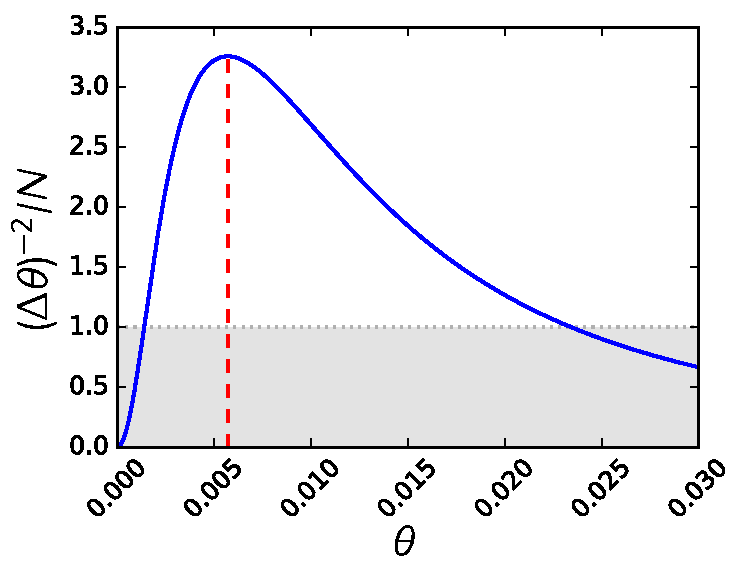
\includegraphics[scale=.65]{img/VD_precision_theta.pdf}
  \caption[Evolution of the precision for $\theta$.]{(solid) The precision as a function of the parameter $\theta$ given by Eq.~\eqref{eq:vd-precision-as-theta} varies through the evolution.
  Note that for the initial moment the precision is zero.
  (dashed) We highlight where the precision reaches its maximum at $\theta \approx 0.0057$.
  (gray-area) It represent the region where the precision is below the shot-noise limit.}
  \label{fig:vd-precision-theta-experiment}
\end{figure}
Since we cannot obtain the expectation value $\expect{J_xJ_y^2J_x}$ we approximate it with the right-hand side of Eq.~\eqref{eq:vd-simplification-of-last-4th-moment}.
With that we underestimate $\varinv{\theta}$.

Thus, we could detect metrological usefulness by measuring the second and fourth moments of the collective angular momentum components.
For future applications of our scheme, it is important to reduce further the number of quantities we need to obtain a lower bound for the precision.
In practice, one can easily avoid the need for determining $\expect{J_y^4}$.
Note that if we measure $J_y$ then the distribution of the values obtained is strongly non-Gaussian.
The values $\pm N/2$ appear most frequently, and the value 0 appears least frequently \cite{Luecke2011}.
See also the distribution of a pure Dicke state when $\theta=\pi/2$ in the Figure~\ref{fig:vd-secuence-evo}.
The state has more overlap with the eigenstates of the edges than in the middle.
Based on $\expect{AB}\leqslant\lambda_{\max}(A)\expect{B}$, where $\lambda_{\max}(A)$ is the largest eigenvalue of $A$, for two commuting positive-semidefinite observables,
\be
  \expect{J_y^4}\leqslant\frac{N^2}{4}\expect{J_x^2}.
\ee
Since even for a noisy Dicke state $\expect{J_y^2}$ is very large, the above equation is a very good upper bound.
Substituting it into the Eq.~\eqref{eq:vd-precision}, we will underestimate $\varinv{\theta}$.

It is also possible to approximate $\expect{J_x^4}$ with $\expect{J_x^2}$ in the sense that it is small and that mainly its value comes from technical noise,
\be
  \expect{J_x^4} \approx \beta \expect{J_x^2}^2.
\ee
This approximation, even if it is not a strict bound on the precision, can be very useful in order to characterize the metrological usefulness of the state based only on second statistical moments of only two angular momentum components, namely $\expect{J_y^2}$ and $\expect{J_x^2}$.
Those two expectation values are related with how  thin is the state in one direction and how wide in the perpendicular ones.
So in this case we use $\beta=3$ assuming that the distribution function has a Gaussian shape.

\begin{figure}[htp]
  \centering
  \igwithlabel{(a)}{scale=.65}{img/VD_exper_contour.pdf}
  \igwithlabel{(b)}{scale=.65}{img/VD_exper_slice.pdf}
  \caption[(a) Precision bound as a function of $\expect{J_y^2}$ and $\expect{J_x^2}$. (b) Precision bound for constant $\expect{J_y^2}$.]{  (a) Precision bound as a function of $\expect{J_y^2}$ and $\expect{J_x^2}$.
  The expectation value $\expect{J_y^2}$ is normalized with $J_{\max}$ or equivalently with $\mathcal{J}_{N/2}$.
  (solid) Different boundaries for metrologically useful entanglement depths are shown with solid lines.
  (cross) and (blue-ellipse) Those elements stand for the point corresponding to the experimental data and the region with one $\sigma$ confidence, respectively.
  (dashed) This corresponds to the constant $\expect{J_y^2}$ cross section plotted next.
  (b) Constant $\expect{J_y^2}$ cross section for the precision bound.
  (solid) Precision bound based on the Eq.~\eqref{eq:vd-precision-bound-for-second-moments}.
  One can see that decreasing further the uncertainty in $\expect{J_x^2}$ can improve the bound significantly.
  (white-point) Experimental data with the corresponding errors.
  Even if the point is slightly below the 4-particle entanglement level, we can say that with only two second moments, we characterize the state in such a way that it does not differ very much from the original prediction when fourth moments were also included and 4-particle entanglement was witnessed for the system.}
  \label{fig:vd-experimental}
\end{figure}
From these considerations we are able to write a second bound with fewer expectation values for the optimal precision such that
\be
  \varian{\theta}_{\text{opt}} \leqslant \frac{\expect{J_y^2} + \frac{3N(N+2)-8}{4} \expect{J_x^2} + \Big(\sqrt{\frac{N^2}{2\expect{J_y^2}}-2} - 2 \Big) \expect{J_y^2}\expect{J_x^2} - 9\expect{J_x^2}^2}
  {4\expect{J_y^2-J_x^2}^2}.
  \label{eq:vd-precision-bound-for-second-moments}
\ee
We have used this formula to compute the bound for the optimal precision with the measured data shown on Eq.~\eqref{eq:vd-experimental-values}, $(\Delta \theta)^{-2}_{\text{opt}} \geqslant 2.9N$, see Figure~\ref{fig:vd-experimental}.
It turns out that even this way, 3-particle metrologically useful entanglement is detected.
Figure~\ref{fig:vd-experimental}-(a) shows the two-dimensional plot which is obtained based on these considerations.
The regions with various levels of multipartite entanglement ca clearly be identified.
The ideal Dicke state corresponds to the bottom-right corner.
In Figure~\ref{fig:vd-experimental}-(b), the cross section of the two-dimensional plot is shown.
